\documentclass[12pt]{extarticle}
\usepackage[margin=1in]{geometry}
\usepackage{amssymb}
\usepackage{amsmath}
\usepackage{url}
\usepackage{bm}
\usepackage{color}
\usepackage{graphicx}

\title{Notes on Siemens Elements of Nuclei}
\author{Cody L. Petrie}

\begin{document}
\maketitle

\setcounter{section}{2}
\section{Scattering by Nuclei}
\subsection{The Black Sphere}
To talk about the scattering of a neutron from some nuclei we are first going to consider scattering from an absorbing spherical object. We start by assuming the incident neutron beam is a plane wave $e^{ikz}$. We then expand this plane wave in terms of legendre polynomials in the scattering regiem.

Expanding a plane wave in the spherical harmonic basis gives
\begin{equation}
   e^{i\mathbf{k}\cdot\mathbf{r}} = \sum\limits_l C_l Y_l^0(\theta).
\end{equation}
There is no $\phi$ dependance here because the plane wave only depend on $\theta$ the angle between $\mathbf{k}$ and $\mathbf{r}$, since the plane wave is propagating in the z direction. Now solving for the expansion coefficients $C_l$ using the orthogonality relationship
\begin{equation}
   \int_0^{\pi} \int_0^{2\pi} Y_l^m Y_{l'}^{m'*} d\Omega = \delta_{ll'}\delta_{mm'},
\end{equation}
gives us
\begin{equation}
   C_l = 2\pi \int_0^{\pi} e^{ikr\cos\theta}Y_l^0(\theta)\sin\theta d\theta.
\end{equation}
Now writting the spherical harmonics in terms of legendre polynomials
\begin{equation}
   Y_l^m(\theta,\phi) = \sqrt{\frac{2l+1(l-m)!}{4\pi(l+m!)}}P_l^m(\cos\theta)e^{im\phi},
\end{equation}
or for $m=0$,
\begin{equation}
   Y_l^0(\theta)=\sqrt{\frac{2l+1}{4\pi}}P_l(\cos\theta)
\end{equation}
we get,
\begin{equation}
   C_l = \pi \int_0^\pi e^{ikr\cos\theta}\sqrt{\frac{2l+1}{4\pi}}P_l(\cos\theta) \sin\theta d\theta.
\end{equation}
Now if you use an identity relating the spherical bessel functions of the first kind to the legendre polynomials (an identity which I found online and proved with Mathematica)
\begin{equation}
   j_l(kr)=\frac{1}{2i^l}\int_0^\pi e^{ikr\cos\theta}P_l{\cos\theta},
\end{equation}
we can get an expansion of the plane wave in terms of spherical bessel functions and legendre polynomials.
\begin{equation}
   \boxed{e^{ikz} = \sum\limits_l 2i^l \sqrt{\pi}\sqrt{2l+1} j_l(kr)Y_l^0(\theta)}
\end{equation}
Often we want to look at these things in the scattering or radiation limit where r is large. We can use the expansion of the spherical bessel function as given by Jackson eq. 9.89 to be
\begin{equation}
   \lim\limits_{r->\infty} j_l(kr) = \frac{1}{kr} \sin\left( kr-\frac{l\pi}{2} \right) = \frac{i}{2kr}(e^{-i(kr-\frac{l\pi}{2}) - e^{i(kr-\frac{l\pi}{2})}}).
\end{equation}
We can thus write the expansion in the asymptotic limit as
\begin{equation}
   \boxed{e^{ikz} \approx \sum\limits_l \frac{\sqrt{\pi}}{kr} \sqrt{2l+1} \, i^{l+1} \left( e^{-i(kr-\frac{l\pi}{2})} - e^{i(kr-\frac{l\pi}{2})} \right) Y_l^0(\theta)}.
\end{equation}
This is equation 3.1.1 in Siemens.


The scattering is going to happen for some finite amount of time while the nucleon interacts with the nucleus and then the scattering interaction will turn off. After the interaction has turned off we can imaging that the amplitude of outgoing wave, $e^{i(kr-\frac{l\pi}{2})}$ has been modified giving us a wave function of
\begin{equation}
   \phi(r\rightarrow\infty) = \sum\limits_l \frac{\sqrt{\pi}}{kr} \sqrt{2l+1} \, i^{l+1} \left( e^{-i(kr-\frac{l\pi}{2})} - \eta_l e^{i(kr-\frac{l\pi}{2})} \right) Y_l^0(\theta).
\end{equation}
Now we can get the scattered wave $\phi_s$ by subtracting the incident plane wave from this since $\phi = \phi_i + \phi_s$.
\begin{align}
   \phi_s &= \sum\limits_l \frac{\sqrt{\pi}}{kr} \sqrt{2l+1} \, i^{l+1} \left( e^{-i(kr-\frac{l\pi}{2})} - \eta_l e^{i(kr-\frac{l\pi}{2})} - e^{-i(kr-\frac{l\pi}{2})} + e^{i(kr-\frac{l\pi}{2})} \right) Y_l^0(\theta) \\
   &= \sum\limits_l \frac{\sqrt{\pi}}{kr} \sqrt{2l+1} \, i^{l+1} e^{i(kr-\frac{l\pi}{2})}(1 - \eta_l) Y_l^0(\theta) \\
   &= \sum\limits_l i \frac{\sqrt{\pi}}{kr} \sqrt{2l+1} e^{ikr}(1 - \eta_l) Y_l^0(\theta) \\
   &= f(\theta) \frac{e^{ikr}}{r}
\end{align}
Where in the last line I have used the face that $i=e^{\pi/2}$, and where
\begin{equation}
   f(\theta) = \sum\limits_l i \frac{\sqrt{\pi}}{k}\sqrt{2l+1} Y_l^0(\theta) (1-\eta_l)
   \label{eq:fullscatamp}
\end{equation}

Putting these together we get
\begin{equation}
   \phi(r\rightarrow\infty) = e^{ikz} + f(\theta)\frac{e^{ikr}}{r},
\end{equation}
where we can recognize the $f(\theta)$ term as being part of the differential scattering cross section, $\frac{d\sigma}{d\Omega} = \left|f(\theta)\right|^2$.

Now let's make some approximations. Siemens says that the classical turning point for a neutron is when $k^2 = l(l+1)/R^2 \approx (l+\frac{1}{2})^2/R^2$. Solving this for l gives $l=kR-\frac{1}{2}$. Now, if a particle passes within the range $R$ then we can say that it is absorbed and $\eta_l=0$. This happens for small angular momentum $l < kR-\frac{1}{2}$. But for large enough angular momentum, $l > kR - \frac{1}{2}$, the particles pass too far away to be scattered and the scattered wave is the same as the incident plane wave, $\eta_l=1$, which gives $\frac{d\sigma}{d\Omega} = 0$, thus we only need to sum to $l=kR-\frac{1}{2}$. Finally this gives us the differential scattering cross section.
\begin{equation}
   \frac{d\sigma}{d\Omega} = \frac{\pi}{k^2} \left|\sum\limits_{l=0}^{kr-1/2} \sqrt{2l+1} Y_l^0(\theta)\right|^2
\end{equation}
The next thing Siemens does is to approximate these for large and small scattering angles. I had a hard time doing the integrals they did so I'll just quote the results here. These are equations 3.1.9a and 3.1.9b in the book.
\begin{align}
   \frac{d\sigma}{d\Omega} \approx
\begin{cases}
   \frac{2R}{\pi} k\theta^2 \sin\theta\cos^2\left(kR\theta+\frac{\pi}{4}\right),& \text{for } kR\theta \gg 1 \\
   \frac{k^2R^4}{4}(1-(kR\theta/2)^2)^2,& \text{for } kR\theta \ll 1
\end{cases}
\label{eq:crossapprox}
\end{align}
I have plotted these two as in figure 3.2 of the book. My reproduction isn't exactly like there's but it is roughly the same.
\begin{figure}[h]
   \centering
   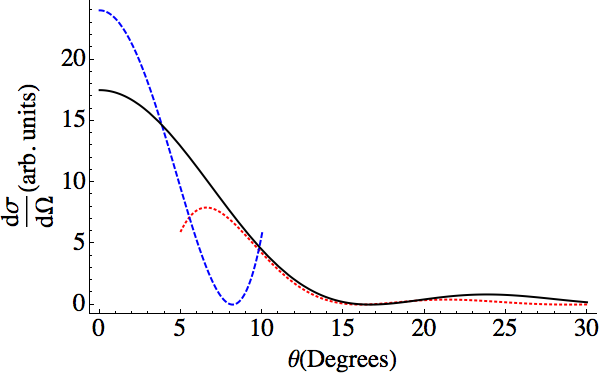
\includegraphics[width=0.5\textwidth]{fig3_2.png}
   \caption{Comparison of approximations where R=7 and k=2. The dashed curve is low angle approximate and the dotted curve is the high angle approximation.}
\end{figure}

\subsection{Nuclear Sizes and the Saturation of Nuclear Forces}
We can use these expressions to learn about the radius of the nucleus. For example if we look for the minimum of the large angle of equation~\ref{eq:crossapprox} we get an expression in terms of the radius.
\begin{align}
   \frac{d}{d\theta}\frac{d\sigma}{d\Omega} &= -\frac{2R}{\pi k\theta^2\sin\theta}2\cos\left(kR\theta+\frac{\pi}{4}\right) + \frac{2R}{\pi k}\cos^2\left(kR\theta+\frac{\pi}{4}\right)\left(-\frac{2}{\theta^3\sin\theta}-\frac{\cos\theta}{\theta^2\sin^2\theta}\right) \\
   &= -\frac{4R}{\pi k\theta^2\sin\theta}\cos\left(kR\theta+\frac{\pi}{4}\right) \left[1 + \cos\left(kR\theta+\frac{\pi}{4}\right)\left(-\frac{1}{\theta}-\frac{1}{2}\frac{\cos\theta}{\sin\theta}\right)\right] \\
\end{align}
This is zero when the argument of the $\cos$ is $n\frac{\pi}{2}$, where n is some integer. So solving $kR\theta+\frac{\pi}{4} = n\frac{\pi}{2}$ we get
\begin{equation}
   \theta_{min} = \frac{\pi}{4kR}(2n-1).
\end{equation}
For some reason (I assume based on where the first minimum in the experimental curves is located) Siemens says that
\begin{equation}
   \boxed{ \theta_{min} = \frac{5\pi}{4kR} }.
\end{equation}
Or equivalently for the nuclear volue $\Omega_r$.
\begin{equation}
   \Omega_r = \frac{4}{3}\pi R^3 = \frac{125}{48}\frac{\pi^4}{(k\theta_{min})^3}
\end{equation}
He then goes to say based on figure 3.1 in his book that if $\epsilon = 84$ MeV for Pb, where $k = \sqrt{2m_n\epsilon/\hbar^2} \approx 2.0$ fm$^{-1}$, and with $\theta_{min} \approx 15^\circ$ you get an esimated radius of lead to be $7.5$ fm. A quick google search shows that the radius is somewhere around $7$ fm.

The book mentions two ways that the spacing between nucleons is districuted among nuclei of different particle numbers ($A$). The first option is like molecules, where the volume is proportional to the number of particles. The second is that for heavier nuclei the nucleus could be squished into tighter radii, where the size of nuclei would be mostly the same regardless of $A$. It turns out that nuclei follow the molecule model better,
\begin{equation}
   \Omega_r = \Omega_0 A
\end{equation}
or
\begin{equation}
   R = r_0 A^{1/3},
\end{equation}
where $r_0 \approx 1.3$ fm or $\Omega_0 = \frac{4}{3} \pi r_0^3 \approx 9$ fm$^3$.
This conparison with molecular forces tells us two things about the force between nucleons. First, the attractive force falls off quickly with separation, and second, The force is repulsive as the nucleons get close enough.

\subsection{The Optical Model}
Now that we have talked about the black sphere model, which accounts for absorption, let's compare this with other models. Let's start with the potential model. We model the motion of the nucleons with a Hamiltonian
\begin{equation}
   H = \frac{\mathbf{p}^2}{2m_N}+U(\mathbf{r}).
\end{equation}
This model does not allow for absorption. The way to compare these two models is to look at the absorption in experiments. We write the total cross section as
\begin{equation}
   \sigma_{tot} = \sigma_{el} + \sigma_{abs}.
\end{equation}
Now look at an attenuation experiment where you pass particles through a targer of thickness $\Delta z$ containing $n$ scatterers per unit volume. For this experiment the emerging intensity, given an incident intensity of $I_0$, is
\begin{equation}
   I = I_0 e^{-\sigma_{tot}n\Delta z}
\end{equation}
Using equation~\ref{eq:fullscatamp} and integrating we can get $\sigma_{el}$.
\begin{align}
   \sigma_{el} &= \int d\Omega \left(\frac{d\sigma}{d\Omega}\right)_{el} \\
   &= \int d\Omega \left|f(\theta)\right|^2 \\
   &= \int d\Omega \left|i\frac{\sqrt{\pi}}{k}\sum\limits_{l=0}^\infty\sqrt{2l+1}(1-\eta_l)Y_l^0(\theta)\right|^2 \\
   &= \frac{\pi}{k^2}\sum\limits_{l=0}^\infty(2l+1)\left|1-\eta_l\right|^2 \int d\Omega\left|Y_l^0(\theta)\right|^2 \\
   &= \frac{\pi}{k^2}\sum\limits_{l=0}^\infty(2l+1)\left|1-\eta_l\right|^2
\end{align}
Here I have used the orthogonality relationship of spherical harmonics again. Now comparing this to the absorbing cross section in the book
\begin{equation}
   \sigma_{abs} = \frac{\pi}{k^2}\sum\limits_{l=0}^\infty(2l+1)\left(1-|\eta_l|^2\right),
\end{equation}
where $(1-|\eta_l|^2)$ is the probability of absorption, we see that these are very close. In fact for the black sphere model where we argued that $\eta_l = 1$ or $0$ we see that they are the same.
\begin{equation}
   \sigma_{el}(\mathrm{black sphere}) = \sigma_{abs}(\mathrm{black sphere}) = \pi R^2
\end{equation}
However, for the potential model $\sigma_{abs}(potential) = 0$ always because it doesn't allow for absorption since the scattering amplitude is unitary.
\begin{equation}
   \eta_l = e^{2i\delta_l}
\end{equation}

Experiments tell us that the cross sections for the elastic and absorptive portions are comparable, thus the potential model needs to be modified. Siemens mentions that since particles are lost or gained in the absorptive process (At least the number of C.M. energy particles) any additional term must not be Hermitian (because probability is not conserved).
\begin{equation}
   H=\frac{\mathbf{p}^2}{2m_H} + U(\mathbf{r}) - iW(\mathbf{r})
\end{equation}
Plugging this into the Schr\"odinger equation for a particle of energy $\epsilon$ traveling in the x direction gives a solution of the form
\begin{equation}
   \phi(\mathbf{r},t) = const \times e^{ikx-\kappa x}e^{-i\epsilon t/\hbar},
\end{equation}
with the conditions
\begin{equation}
   \frac{\hbar^2}{2m_N}(k^2-\kappa^2) = \epsilon - U
\end{equation}
and
\begin{equation}
   \frac{\hbar^2}{m_N}\kappa k = W
   \label{eq:Wwithkappa}
\end{equation}
From this we can determine the mean free path by noting that the probability density goes as
\begin{equation}
   \left|\phi(\mathbf{r})\right|^2 \sim e^{-2\kappa x}
\end{equation}
which falls off by $1/e$ at the mean free path of
\begin{equation}
   \lambda = \frac{1}{2\kappa}.
   \label{eq:meanfreepath}
\end{equation}

Of course we know that there should be spin dependant pieces to the Hamiltonian and so we include a spin-orbit term and call it the \textbf{Phenomenological Optical Model}. The optical model is given this name for the fact that it allows for partial absorption and partial transmission of an incident beam, like in optics.
\begin{align}
   H^{POM}=\frac{\mathbf{p}^2}{2m_H} + U(r) + \mathbf{l}\cdot\mathbf{s}U^{ls}(r) - iW(r)
\end{align}
The book mentions that this is then solved similarly to the way in which we solved previously for the scattering and then fit to scattering data in different angular momentum channels. This gives us the potentials
\begin{align}
   U(r) &= U_0f((r-R(A))/r_u)+U_C(r) \\
   W(r) &= \left(W_0-4W_1a_W\frac{\partial}{\partial r}\right)f((r-R(A))/a_W) \\
   U^{ls}(r) &= U^{ls}_0\frac{1}{r}\frac{\partial}{\partial r}f((r-R(A))/a_{ls}).
\end{align}
Here $U_C(r)$ is the Coulomb potential and only effects protons, and 
\begin{align}
   f(x) &= (1+e^{x})^{-1} \\
   R(A) &= r_0 A^{1/3},
\end{align}
and
\begin{align}
   r_0 &= 1.25 \mathrm{fm} \\
   a_u &= 0.65 \mathrm{fm} \\
   a_{ls} &= a_W = 0.47 \mathrm{fm}.
\end{align}
The function $f$ is called the \textbf{Woods-Saxon shape} and is plotted for various values of $A$ in figure~\ref{fig:woodssaxon}.
\begin{figure}[h]
   \centering
   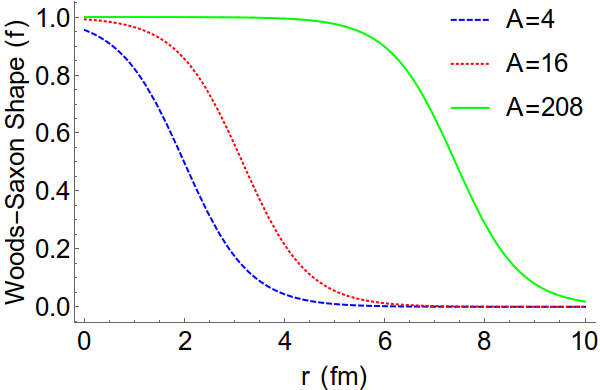
\includegraphics[width=0.5\textwidth]{woodssaxon.png}
   \caption{Woods-Saxon shape plotted for A=4,16,208.}
   \label{fig:woodssaxon}
\end{figure}
Notice how it approaches 1 inside the nuclei and falls from 0.9 to 0.1 as $r$ varies from $R-2.2a_U$ to $R+2.2a_U$. Siemens says that the nucleus has a \textbf{uniform interior}, and a \textbf{surface thickness} of $4.4a_u$, which is about 2.9 fm (about the range of the force). Also, it turns out that the parameters $W_0, W_1$, and $U_0$ depend on the energy of the incident nucleon ($\epsilon$).
\begin{align}
   W_0(\epsilon) &\approx \max (0.22\epsilon - 2\mathrm{MeV},0) \\
   W_1(\epsilon) &\approx \max \left[12\mathrm{MeV} - 0.25\epsilon + 24\mathrm{MeV} \cdot t_3\frac{N-Z}{A},0\right] \\
   U_0(\epsilon) &\approx -50\mathrm{MeV}-48\mathrm{MeV}\cdot t_3\frac{N-Z}{A}+0.3(\epsilon-U_C(R)) \\
   U_0^{ls} &\approx 30\mathrm{MeV fm^2/\hbar^2}
\end{align}
\begin{figure}[h]
   \centering
   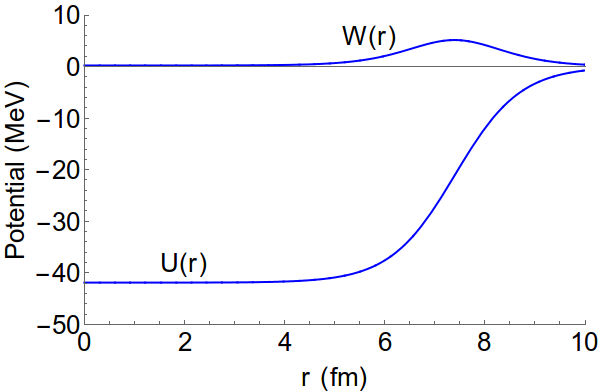
\includegraphics[width=0.5\textwidth]{fig3_3.png}
   \caption{Phenomenological optical potential of a 10 MeV neutron in ${}^{208}$Pb.}
   \label{fig:phenpot}
\end{figure}

Looking at this Hamiltonian we recognize that it's more like the $\mathcal{T}$ matrix that we encountered in chapter 2 than a true Hamiltonian. It doesn't conserve probability and it depends on the energy. We will see the connection next chapter between the $\mathcal{T}$ and the optical Hamiltonian.

One last riddle the book mentions is in relation to the magnitude of $W_0$. Using equations~\ref{eq:Wwithkappa} and \ref{eq:meanfreepath} the mean free path is of a 40 MeV neutron is estimated to be 5 fm, where the $\lambda = (n\sigma)^{-1} \approx 0.4$ fm, where $\sigma \approx 4\pi d\sigma/d\Omega$, and $n=(4\pi r_0^3/3)^{-1}$. This is off by a factor of about 10. This riddle will be solved in chapter 4.

\subsection{Nuclear Matter}
Given the success of this model it is appropriate to think of a nucleus of a uniform center surrounded by a surface that is about one particle thick. This uniform center, that exists in all nuclei, can be though of as a drop of nuclear matter.

It is convenient then to sometimes think of these nuclear centers extending on forever (obviously having to neglect the Coulomb interaction which pushed the nucleus apart). This can make calculations easier. One way in which this is made easier is in the fact that correlations which depend on the coordinates of two particles, $\mathbf{r_1}$ and $\mathbf{r_2}$, now only depend on one coordinate, the differenct $\mathbf{r_1}-\mathbf{r_2}$ because of translational invariance.

\subsection{Electromagnetic Forces; Scattering of Electrons and Protons by Nuclei}
To experimentally learn about the the electrostatic potential it is convenient to scatter electrons rather than protons from a nucleus, since the electron will not feel the nuclear force. This can be done within the born approximation in the usual way, by making the interaction (electrostatic) smaller than the kinetic energy.

It turns out that the shape of the charge distribution is similar to the optical potential and thus can be fit the the Woods-Saxon shape. If fit to this shape the thickness is about $0.55$ fm, and the radius is about $R(A) \approx 1.15 ~\mathrm{fm}A^{1/3}$. These numbers are a little smaller than the equivalent values for the potential. It makes sence that the potential reaches farther than the charge density.

Handling this coulomb potential is tedious theoretically because of its long range, but it is at least straight forward.

\subsection{Scattering of Pions by Nuclei}
Figure 3.5 in the book shows the differential cross section of negative pions scattering from ${}^{12}C$ and shows the same diffractive pattern seen before. So here there is also both elastic and absorptive scattering. Before we said that something was absorbed if the enregy changed from the C.M. energy, but with pions the final state may not contain any pions, and so it true absorption.

To be able to conserve both energy and momentum you have to have at least two nucleons in the scattering process. The first nucleon will absorb the pion and create a delta. Then the delta will scatter inelastically with the second nucleon creating two nucleons again.

\end{document}
